\iffalse
This file is protected by Copyright. Please refer to the COPYRIGHT file
distributed with this source distribution.

This file is part of OpenCPI <http://www.opencpi.org>

OpenCPI is free software: you can redistribute it and/or modify it under the
terms of the GNU Lesser General Public License as published by the Free Software
Foundation, either version 3 of the License, or (at your option) any later
version.

OpenCPI is distributed in the hope that it will be useful, but WITHOUT ANY
WARRANTY; without even the implied warranty of MERCHANTABILITY or FITNESS FOR A
PARTICULAR PURPOSE. See the GNU Lesser General Public License for more details.

You should have received a copy of the GNU Lesser General Public License along
with this program. If not, see <http://www.gnu.org/licenses/>.
\fi

%----------------------------------------------------------------------------------------
% Required document specific properties
%----------------------------------------------------------------------------------------
\def\comp{pattern\_{}v2}
\edef\ecomp{pattern_v2}
\def\Comp{Pattern v2}
\def\docTitle{\Comp{} Component Data Sheet}
\def\snippetpath{../../../../../../doc/av/tex/snippets}
%----------------------------------------------------------------------------------------
% Global latex header (this must be after document specific properties)
%----------------------------------------------------------------------------------------
\iffalse
This file is protected by Copyright. Please refer to the COPYRIGHT file
distributed with this source distribution.

This file is part of OpenCPI <http://www.opencpi.org>

OpenCPI is free software: you can redistribute it and/or modify it under the
terms of the GNU Lesser General Public License as published by the Free Software
Foundation, either version 3 of the License, or (at your option) any later
version.

OpenCPI is distributed in the hope that it will be useful, but WITHOUT ANY
WARRANTY; without even the implied warranty of MERCHANTABILITY or FITNESS FOR A
PARTICULAR PURPOSE. See the GNU Lesser General Public License for more details.

You should have received a copy of the GNU Lesser General Public License along
with this program. If not, see <http://www.gnu.org/licenses/>.
\fi

% Sets OpenCPI Version used throughout all the docs. This is updated by
% scripts/update-release.sh when a release is being made and must not
% be changed manually.
\def\ocpiversion{v2.2.0}

\documentclass{article}
\author{}  % Force author to be blank
\date{OpenCPI Release:\ \ \ocpiversion}  % Force date to be blank and override date with version
\title{OpenCPI\\\docTitle}  % docTitle must be defined before including this file
%----------------------------------------------------------------------------------------
% Paper size, orientation and margins
%----------------------------------------------------------------------------------------
\usepackage{geometry}
\geometry{
  letterpaper,  % paper type
  portrait,     % text direction
  left=.75in,   % left margin
  top=.75in,    % top margin
  right=.75in,  % right margin
  bottom=.75in  % bottom margin
}
%----------------------------------------------------------------------------------------
% Header/Footer
%----------------------------------------------------------------------------------------
\usepackage{fancyhdr} \pagestyle{fancy}  % required for fancy headers
\renewcommand{\headrulewidth}{0.5pt}
\renewcommand{\footrulewidth}{0.5pt}
\lhead{\small{\docTitle}}
\rhead{\small{OpenCPI}}
%----------------------------------------------------------------------------------------
% Various packages
%----------------------------------------------------------------------------------------
\usepackage{amsmath}
\usepackage[page,toc]{appendix}  % for appendix stuff
\usepackage{enumitem}
\usepackage{graphicx}   % for including pictures by file
\usepackage{hyperref}   % for linking urls and lists
\usepackage{listings}   % for coding language styles
\usepackage{pdflscape}  % for landscape view
\usepackage{pifont}     % for sideways table
\usepackage{ragged2e}   % for justify
\usepackage{rotating}   % for sideways table
\usepackage{scrextend}
\usepackage{setspace}
\usepackage{subfig}
\usepackage{textcomp}
\usepackage[dvipsnames,usenames]{xcolor}  % for color names see https://en.wikibooks.org/wiki/LaTeX/Colors
\usepackage{xstring}
\uchyph=0  % Never hyphenate acronyms like RCC
\renewcommand\_{\textunderscore\allowbreak}  % Allow words to break/newline on underscores
%----------------------------------------------------------------------------------------
% Table packages
%----------------------------------------------------------------------------------------
\usepackage[tableposition=top]{caption}
\usepackage{float}
\floatstyle{plaintop}
\usepackage{longtable}  % for long possibly multi-page tables
\usepackage{multicol}   % for more advanced table layout
\usepackage{multirow}   % for more advanced table layout
\usepackage{tabularx}   % c=center,l=left,r=right,X=fill
% These define tabularx columns "C" and "R" to match "X" but center/right aligned
\newcolumntype{C}{>{\centering\arraybackslash}X}
\newcolumntype{M}[1]{>{\centering\arraybackslash}m{#1}}
\newcolumntype{P}[1]{>{\centering\arraybackslash}p{#1}}
\newcolumntype{R}{>{\raggedleft\arraybackslash}X}
%----------------------------------------------------------------------------------------
% Block Diagram / FSM Drawings
%----------------------------------------------------------------------------------------
\usepackage{tikz}
\usetikzlibrary{arrows,decorations.markings,fit,positioning,shapes}
\usetikzlibrary{automata}  % used for the fsm
\usetikzlibrary{calc}      % for duplicating clients
\usepgfmodule{oo}          % to define a client box
%----------------------------------------------------------------------------------------
% Colors Used
%----------------------------------------------------------------------------------------
\usepackage{colortbl}
\definecolor{blue}{rgb}{.7,.8,.9}
\definecolor{ceruleanblue}{rgb}{0.16, 0.32, 0.75}
\definecolor{cyan}{rgb}{0.0,0.6,0.6}
\definecolor{darkgreen}{rgb}{0,0.6,0}
\definecolor{deepmagenta}{rgb}{0.8, 0.0, 0.8}
\definecolor{maroon}{rgb}{0.5,0,0}
%----------------------------------------------------------------------------------------
% Define where to hyphenate
%----------------------------------------------------------------------------------------
\hyphenation{Cent-OS}
\hyphenation{install-ation}
%----------------------------------------------------------------------------------------
% Define Commands & Rename Commands
%----------------------------------------------------------------------------------------
\newcommand{\code}[1]{\texttt{#1}}  % For inline code snippet or command line
\newcommand{\sref}[1]{Section~\ref{#1}}  % To quickly reference a section
\newcommand{\todo}[1]{\textcolor{red}{TODO: #1}\PackageWarning{TODO:}{#1}}  % To do notes
\renewcommand{\contentsname}{Table of Contents}
\renewcommand{\listfigurename}{List of Figures}
\renewcommand{\listtablename}{List of Tables}

% This gives a link to gitlab.io document. By default, it outputs the filename.
% You can optionally change the link, e.g.
% \githubio{FPGA\_Vendor\_Tools\_Installation\_Guide.pdf} vs.
% \githubio[\textit{FPGA Vendor Tools Installation Guide}]{FPGA\_Vendor\_Tools\_Installation\_Guide.pdf}
% or if you want the raw ugly URL to come out, \githubioURL{FPGA_Vendor_Tools_Installation_Guide.pdf}
\newcommand{\githubio}[2][]{% The default is for FIRST param!
\href{http://opencpi.gitlab.io/releases/\ocpiversion/docs/#2}{\ifthenelse{\equal{#1}{}}{\texttt{#2}}{#1}}}
\newcommand{\gitlabcom}[2][]{% The default is for FIRST param!
\href{http://gitlab.com/opencpi/#2}{\ifthenelse{\equal{#1}{}}{\texttt{#2}}{#1}}}
\newcommand{\githubioURL}[1]{\url{http://opencpi.gitlab.io/releases/\ocpiversion/docs/#1}}
% Lastly, if you want a SINGLE leading path stripped, e.g. assets/X.pdf => X.pdf:
\newcommand{\githubioFlat}[1]{%
\StrBehind{#1}{/}[\den]%
\href{http://opencpi.gitlab.io/releases/\ocpiversion/docs/#1}{\texttt{\den}}%
}
%----------------------------------------------------------------------------------------
% VHDL Coding Language Style
% modified from: http://latex-community.org/forum/viewtopic.php?f=44&t=22076
%----------------------------------------------------------------------------------------
\lstdefinelanguage{VHDL}
{
  basicstyle=\ttfamily\footnotesize,
  columns=fullflexible,keepspaces,  % https://tex.stackexchange.com/a/46695/87531
  keywordstyle=\color{ceruleanblue},
  commentstyle=\color{darkgreen},
  morekeywords={
    library, use, all, entity, is, port, in, out, end, architecture, of,
    begin, and, signal, when, if, else, process, end,
  },
  morecomment=[l]--
}
%----------------------------------------------------------------------------------------
% XML Coding Language Style
% modified from http://tex.stackexchange.com/questions/10255/xml-syntax-highlighting
%----------------------------------------------------------------------------------------
\lstdefinelanguage{XML}
{
  basicstyle=\ttfamily\footnotesize,
  columns=fullflexible,keepspaces,
  morestring=[s]{"}{"},
  morecomment=[s]{!--}{--},
  commentstyle=\color{darkgreen},
  moredelim=[s][\color{black}]{>}{<},
  moredelim=[s][\color{cyan}]{\ }{=},
  stringstyle=\color{maroon},
  identifierstyle=\color{ceruleanblue}
}
%----------------------------------------------------------------------------------------
% DIFF Coding Language Style
% modified from http://tex.stackexchange.com/questions/50176/highlighting-a-diff-file
%----------------------------------------------------------------------------------------
\lstdefinelanguage{diff}
{
  basicstyle=\ttfamily\footnotesize,
  columns=fullflexible,keepspaces,
  breaklines=true,                            % wrap text
  morecomment=[f][\color{ceruleanblue}]{@@},  % group identifier
  morecomment=[f][\color{red}]-,              % deleted lines
  morecomment=[f][\color{darkgreen}]+,        % added lines
  morecomment=[f][\color{deepmagenta}]{---},  % Diff header lines (must appear after +,-)
  morecomment=[f][\color{deepmagenta}]{+++},
}
%----------------------------------------------------------------------------------------
% Python Coding Language Style
%----------------------------------------------------------------------------------------
\lstdefinelanguage{python}
{
  basicstyle=\ttfamily\footnotesize,
  columns=fullflexible,keepspaces,
  keywordstyle=\color{ceruleanblue},
  commentstyle=\color{darkgreen},
  stringstyle=\color{orange},
  morekeywords={
    print, if, sys, len, from, import, as, open,close, def, main, for, else,
    write, read, range,
  },
  comment=[l]{\#}
}
%----------------------------------------------------------------------------------------
% Fontsize Notes in order from smallest to largest
%----------------------------------------------------------------------------------------
%    \tiny
%    \scriptsize
%    \footnotesize
%    \small
%    \normalsize
%    \large
%    \Large
%    \LARGE
%    \huge
%    \Huge

%----------------------------------------------------------------------------------------

\begin{document}
\maketitle
\thispagestyle{empty}
\newpage

\begin{center}
\textit{\textbf{Revision History}}
	\begin{table}[H]
	\label{table:revisions} % Add "[H]" to force placement of table
		\begin{tabularx}{\textwidth}{|c|X|l|}
			\hline
			\rowcolor{blue}
			\textbf{Revision} & \textbf{Description of Change} & \textbf{Date} \\
		    \hline
		    v1.4 & Initial Release & 10/2018 \\
		    \hline
			v1.5 & \begin{itemize} \item Fixed incorrect property accessibility "Writable" and changed it to "Initial" for the \texttt{messagesToSend} property. \item Clarified that the opcode that is sent by the component is an 8 bit opcode. \end{itemize} & 4/2019 \\
			\hline
			v1.6 & Converted Worker to version 2 & 11/2019 \\
			\hline
			v1.7 & Table of Worker Configurations and Resource Utilization Table removed & 5/2020 \\
			\hline
			v2.2 & {\Comp} updated to use input port clock. RCC version of \comp created. Functionality of messagesToSend slightly changed/improved.  & 7/2021 \\
	                \hline
		\end{tabularx}
	\end{table}
\end{center}
\newpage

\def\name{\comp}
\def\workertype{}
\def\version{\ocpiversion}
\def\releasedate{05/2020}
\def\componentlibrary{ocpi.assets.util\_{}comps}
\def\workers{\comp{}.hdl}
\def\testedplatforms{isim, Matchstiq-Z1(PL), xsim, ZedBoard(PL), centos 7}
\section*{Summary - \Comp}
\begin{tabular}{|c|M{13.5cm}|}
  \hline
  \rowcolor{blue}
   & \\
  \hline
  Name              & \comp             \\
  \hline
  Worker Type       & \workertype       \\
  \hline
  OpenCPI Release   & \ocpiversion      \\
  \hline
  Last Update       & \releasedate      \\
  \hline
  Component Library & \componentlibrary \\
  \hline
  Workers           & \workers          \\
  \hline
  Tested Platforms  & \testedplatforms  \\
  \hline
\end{tabular}

	
\section*{Functionality}
\begin{flushleft}

The {\comp} component provides the ability to output a pattern of messages by allowing the user to create a record of messages each having a configurable number of bytes and associated 8 bit opcode. Through a set of properties, the component may send messages (data and opcode) up to the amount dictated by the build-time parameters. \newline

The \texttt{messages} property defines the record of messages to send, as well as, defines the number of data bytes and an opcode for each message. \newline

For example: \newline

When \texttt{messages} = \{4, 255\}, one message will be sent having 4 bytes of data and an opcode of 255. \newline
When \texttt{messages} = \{8, 251\}, \{12, 250\}, two messages will be sent, the first having 8 bytes of data and an opcode of 251, and the second message having 12 bytes of data and an opcode of 250. \newline

Data to be sent with a message is defined by the \texttt{data} property and is referred to as the data buffer. The number of data words in the data buffer is the number of data bytes for the messages. \newline

The component offers an additional feature when there are multiple messages via the \texttt{dataRepeat} property which indicates whether the a message starts at the beginning of the data buffer, or continues from its current index within the buffer. \newline

For example: \newline

Given \texttt{messages} = \{4, 251\},\{8, 252\},\{12, 253\},\{16, 254\},\{20, 255\} \newline

If \texttt{dataRepeat} = true, then \texttt{numDataWords} is 5. To calculate the \texttt{numDataWords} when \texttt{dataRepeat} is true, divide the largest message size (in bytes) by 4. Dividing by four required because the data is output as a 4 byte data word. Since the largest message size in the given messages assignment is 20, 20/4 = 5. \newline

When \texttt{numDataWords} = 5, then a valid data assignment would be \texttt{data} = \{0, 1, 2, 3, 4\}, and the data within each message would look like:
msg1 = \{0\}, msg2 = \{0, 1\}, msg3 = \{0, 1, 2\}, msg4 = \{0, 1, 2, 3\}, msg5 = \{0, 1, 2, 3, 4\}  \newline

If \texttt{dataRepeat} = false, then \texttt{numDataWords} is 15. To calculate the \texttt{numDataWords} when \texttt{dataRepeat} is false, divide the sum of all the message sizes (in bytes) by 4. Dividing by four is required because the data is output as a 4 byte data word. Since the sum of all message sizes in the given messages assignment is (4+8+12+16+20)/4 = 15. \newline

When \texttt{numDataWords} = 15, then a valid data assignment would be \texttt{data} = \{0, 1, 2, 3, 4, 5, 6, 7, 8, 9, 10, 11, 12, 13, 14\}, and the data within each message would look like: msg1 = \{0\}, msg2 = \{1, 2\}, msg3 = \{3, 4, 5\}, msg4 = \{6, 7, 8, 9\}, msg5 = \{10, 11, 12, 13, 14\}  \newline

There is also a \texttt{messagesToSend} property that sets the number of messages to send and decrements as the messages are sent. When \texttt{dataRepeat} is true, messagesToSend > numMessagesMax, and at the end of the messages buffer, the buffer wraps around and starts at the beginning of the messages buffer. When \texttt{dataRepeat} is false, this value must be less than or equal to \texttt{numMessagesMax}. The HDL and RCC worker will check for this and report an error if \texttt{messagesToSend} is greater than \texttt{numMessagesMax}. The error checking for the HDL worker only happens in simulation.  \newline

When using {\comp}.hdl, the \texttt{messagesToSend}, \texttt{messagesSent},  and \texttt{dataSent} properties should be checked at the end of an app run because they won't be stable until then. The worker doesn't use cdc crossing circuits for them because it takes advantage that they will have a stable value by the time the control plane reads those values at the end of an app run.


\end{flushleft}

\section*{Block Diagrams}
	\subsection*{Top level}
\begin{center}
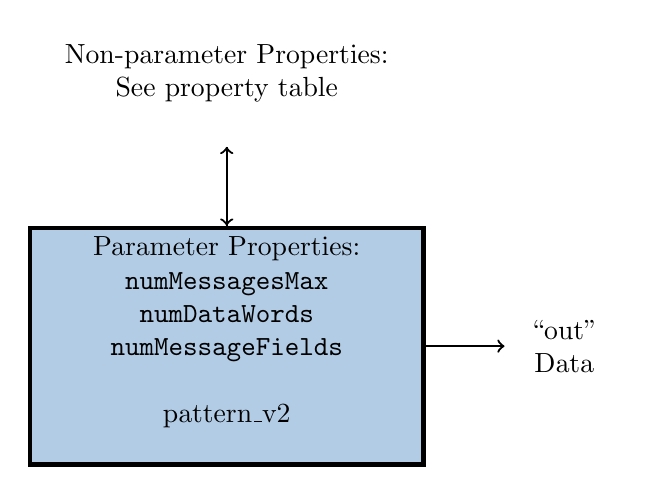
\begin{tikzpicture}[% List of styles applied to all, to override specify on a case-by-case
					every node/.style={
						align=center,  		% use this so that the "\\" for line break works
						minimum size=1.5cm	% creates space above and below text in rectangle
						},
					every edge/.style={draw,thick}
					]
\node[rectangle,ultra thick,draw=black,fill=blue, minimum width=5 cm](R2){Parameter Properties:\\ \verb+numMessagesMax+ \\ \verb+numDataWords+ \\ \verb+numMessageFields+ \\ \\ \comp \\ };
\node[rectangle,draw=white,fill=white](R3)[right= of R2]{``out'' \\ Data};
\node[rectangle,draw=white,fill=white](R4)[above= of R2]{Non-parameter Properties: \\ See property table \\};
\path[->]
(R2)edge []     node [] {} (R3)
(R2)edge []     node [] {} (R4)
(R4)edge []     node [] {} (R2)
;
\end{tikzpicture}
\end{center}

\section*{Source Dependencies}
\subsection*{\comp.hdl}
	\begin{itemize}
		\item assets/components/util\_comps/\comp.hdl/\comp.vhd
		\item core/hdl/primitives/util/BRAM2.v
		\item core/hdl/primitives/util/util\_pkg.vhd
	\end{itemize}

\subsection*{\comp.hdl}
	\begin{itemize}
		\item assets/components/util\_comps/\comp.rcc/\comp.cc
	\end{itemize}

\begin{landscape}
\section*{Component Spec Properties}

\begin{flushleft}

        \begin{scriptsize}
        \begin{tabular}{|p{2.5cm}|p{1cm}|p{1.5cm}|p{2cm}|p{2cm}|p{2.5cm}|p{1.5cm}|p{1.5cm}|p{5.5cm}|}
                \hline
                \rowcolor{blue}
                Name & Type & Default & SequenceLength & ArrayLength & ArrayDimensions & Parameter  & Accessibility & Usage \\
                \hline
                \verb+dataRepeat+ & bool & false & - & - & - & false & Initial & True -  Multiple messages sent from the beginning of the data buffer. \newline
False - Multiple messages sent from the current position of the data buffer.\\
                \hline
                \verb+numMessagesMax+ & uLong & 5 & - & - & - & true & - & Max number of messages to send.  \\
                \hline
                \verb+messagesToSend+ & uLong & 5 & - & - & - & false & Volatile, Initial & Counter of messages to send and decrements as they are sent. When dataRepeat is true, 
    messagesToSend > numMessagesMax, and at the end of the messages buffer, the buffer wraps around and starts at the beginning of the messages buffer. When dataRepeat is false, 
    this value must be less than or equal to numMessagesMax. \\
                \hline
                \verb+messagesSent+ & uLong & - & - & - & - & false & Volatile & Messages sent counter. Initialized to 0.\\
                \hline
                 \verb+dataSent+ & uLong & - & - & - & - & false & Volatile & Words sent counter. Initialized to 0. \\
                \hline
                \verb+numDataWords+ & uLong & 15 & - & - & - & true & - & Max number of four byte data for the data buffer.   To calculate the numDataWords when dataRepeat is true, divide the largest message size (in bytes) by 4. To calculate the numDataWords when dataRepeat is false, divide the sum of all the message sizes (in bytes) by 4. Dividing by four required because the data is output as a 4 byte data word. \\
                \hline
                \verb+numMessageFields+ & uLong & 2 & - & - & - & true & - & Due to a limitation, cannot use constrained elements in unconstrained array declarations, so cannot directly set the second dimension for the messages property to 2. The numMessageFields property must always be 2 since there are 2 message fields; the number of data bytes and opcode. So the default value must not be changed.  \\
                \hline
                \verb+messages+ & uLong & - & - & - & numMessagesMax, numMessageFields & false & Initial & Multidimensional array that defines the record of messages to send, as well as, defines the number of data bytes and an 8 bit opcode for each message.\\
                \hline
                \verb+data+ & uLong & - & - & numDataWords & - & false & Initial & Data buffer containing the data to be sent.\\
                \hline
        \end{tabular}
        \end{scriptsize}


\end{flushleft}


\section*{Component Ports}

        \begin{scriptsize}
                \begin{tabular}{|M{2.5cm}|M{2cm}|M{2cm}|M{2.5cm}|M{12.5cm}|}
                        \hline
                        \rowcolor{blue}
                        Name & Protocol & Producer & Optional & Usage\\
                        \hline
                        out
                        & -
                        & true
                        & false
                        & Data generated by the component \\
                        \hline
                \end{tabular}
			\end{scriptsize}

\section*{Worker Interfaces}
\subsection*{\comp.hdl}
\begin{scriptsize}
\begin{tabular}{|M{2.5cm}|M{2.5cm}|M{3.5cm}|c|M{3.5cm}|M{3.5cm}|}
            \hline
            \rowcolor{blue}
            Type    & Name & DataWidth (b) & Advanced  & Usage     \\
            \hline
            StreamInterface & out   & 32  & DataValueWidth=8, NumberOfOpcodes='256', ZeroLengthMessages=true, clockDirection="in"  & Data generated by the worker \\
           \hline
\end{tabular}
\end{scriptsize}
\end{landscape}

\section*{Control Timing and Signals}
\begin{flushleft}
The {\comp} worker uses the clock from the Data Plane and Control Plane. And it uses standard Control Plane signals.
\end{flushleft}

\begin{landscape}
\section*{Worker Configuration Parameters}
\subsubsection*{\comp.hdl}
%\input{../../\ecomp.hdl/configurations.inc}
\section*{Performance and Resource Utilization}
\subsubsection*{\comp.hdl}
%\input{../../\ecomp.hdl/utilization.inc}
\end{landscape}


\section*{Test and Verification}
\normalsize

\begin{flushleft}

The {\comp} worker is tested by generating data for the \texttt{messages} and \texttt{data} properties and verifying that final value of the volatile properties and the output data are correct. Since the {\comp} worker's \texttt{messages} and \texttt{data} property array sizes depend on parameters, they have to be generated via scripts(\path{gen_messages.py} and \path{gen_data.py})
\newline


\end{flushleft}

\section*{Applications}
\begin{flushleft}

For an example of the {\comp} component used in an application, please reference the
tb\_bias\_v2 application located in \path{assets/applications/tb_bias_v2}.

\end{flushleft}

\end{document}
